\documentclass[xcolor=table]{beamer}

\usepackage{lscape, amsmath, amsfonts, amssymb, setspace, theorem, wrapfig, graphicx, float, multirow, subfig, color, rotating, multicol, datetime, natbib, venndiagram, pstricks, xkeyval, tikz, etoolbox}

\title{GV300 - Quantitative Political Analysis}
\subtitle{University of Essex - Department of Government}
\date{Week 5 -- 28 October, 2019}				% or you can specify a date, just write it down instead of "\today"
\author{Lorenzo Crippa} 

\usetheme[progressbar=frametitle]{metropolis}
\usecolortheme{seahorse}						% try others: wolverine; crane...

\begin{document}
\frame{
\titlepage
}

\frame{
\frametitle{Your GTA}

\begin{center}
Hi! My name is Lorenzo Crippa,

Email: l.crippa@essex.ac.uk

Office: 5B.153 (Department of Government)

Office hour: Wednesday 14:00 to 16:00
\end{center}
}

\frame{
\frametitle{Problem Set 1 -- Answers provided by Dominik Duell}

\begin{center}
Start from problem number 5: Introduce ourselves
\end{center}

\begin{enumerate}
\item What topic you want to be working on?
\item Why this topic is relevant and important to do research on? 
\item The research question you aim to answer? 
\item How you would try to answer this question? (Refer to which kind of experiment you would try to run, data you would need to collect, and/or how you would analyze this data)
\item What you expect the answer to your research question might be?
\end{enumerate}
}

\frame{
\frametitle{Problem 1}
Use Venn Diagrams (or operations on sets) to determine which of the following is true (24 marks, 6 each): 

\begin{itemize}
\item[(a)] $(A+B+C)' = A'+B'+C'$ is not true.
{\footnotesize
\begin{multicols}{2}
\begin{center}$(A+B+C)'=(A\cup B\cup C)'$\end{center}
\scalebox{.6}{\begin{venndiagram3sets}
	\fillNotABC
\end{venndiagram3sets}}

\begin{center}$A'+B'+C'=A'\cup B'\cup C'$\end{center}
\scalebox{.6}{\begin{venndiagram3sets}
	\fillNotA \fillNotB \fillNotC
\end{venndiagram3sets}}
\end{multicols}
}
\end{itemize}
}

\frame{
\frametitle{Problem 1}
\begin{itemize}
\item[(b)] $A + B + C = A + A'B + (A + A'B)'C$ is true.
{\footnotesize
\begin{multicols}{2}
\begin{center}$A+B+C=A\cup B\cup C$\end{center}
\scalebox{.6}{\begin{venndiagram3sets}
	\fillA \fillB \fillC
\end{venndiagram3sets}}

\begin{center}$A + A'B + (A + A'B)'C$\end{center}
\scalebox{.6}{\begin{venndiagram3sets}
	\fillA \fillB \fillC
\end{venndiagram3sets}}
\end{multicols}
}
\end{itemize}
}

\frame{
\frametitle{Problem 1}
\begin{itemize}
\item[(c)] $(A + B)(A'+B') = AB' + A'B + A'BC'$ is true.
{\footnotesize
\begin{multicols}{2}
\begin{minipage}{3cm}
\begin{center}$(A + B)(A'+B')=(A\cup B)\cap(A'\cup B')$\vspace{.4cm}\end{center}
\scalebox{.6}{\begin{venndiagram3sets}
	\fillANotB \fillBNotA
\end{venndiagram3sets}}
\end{minipage}

\begin{minipage}{3cm}
\begin{center}$AB' + A'B + A'BC'=(A\cap B')\cup (A'\cap B) \cup (A'\cap B\cap C')$\end{center}
\scalebox{.6}{\begin{venndiagram3sets}
	\fillANotB \fillBNotA
\end{venndiagram3sets}}
\end{minipage}
\end{multicols}
}
\end{itemize}
}

\frame{
\frametitle{Problem 1}
\begin{itemize}
\item[(d)] $AB + AB' + A'B = (A'B')'$ is true. 
{\footnotesize
\begin{multicols}{2}
\begin{minipage}{3cm}
\begin{center}$AB + AB' + A'B=(A\cap B)\cup(A\cap B')\cup(A'\cap B)$\end{center}
\scalebox{.6}{\begin{venndiagram3sets}
	\fillACapB \fillANotB \fillBNotA
\end{venndiagram3sets}}
\end{minipage}

\begin{minipage}{3cm}
\begin{center}$(A'B')'=(A'\cap B')'$\vspace{.8cm}\end{center}
\scalebox{.6}{\begin{venndiagram3sets}
	\fillA \fillB
\end{venndiagram3sets}}
\end{minipage}
\end{multicols}
}
\end{itemize}
}

\frame{
\frametitle{Problem 2}
Consider an experiment where you throw two three-sided dice. Let $F_n$ be the event ``The first die rolls an n'' and $S_n$ be ``The second die rolls an n.'' Determine whether each of the following are mutually exclusive, collectively exhaustive, a sample space or an event space. Which set of descriptors apply to each (24 marks, 6 each)?
}

\frame{
\frametitle{Problem 2 -- About the sample space}
\begin{center}
Who knows what a ``sample space'' is? 
\end{center}
}

\frame{
\frametitle{Problem 2 -- About the sample space}
\begin{itemize}
\item A ``sample space'' represents all possible outcomes. \\
\item It is defined over outcomes, {\bf not} events. \\
\item Problem 2 presents collections of events. The concept of ``sample space'' does not apply to them
\item The following statement can never be true: ``This collection of {\bf events} can be described as a sample space.
\item Sample space: \{$F_1$,$S_1$; $F_1$,$S_2$; $F_1$,$S_3$; $F_2$,$S_1$; $F_2$,$S_2$; $F_2$,$S_3$; $F_3$,$S_1$; $F_3$,$S_2$; $F_3$,$S_3$\}  
\end{itemize}
}

\frame{
\frametitle{Problem 2}
\begin{enumerate}
\item[(a)] $F_1$; $F_2$; $(F1 \cup F2)'$
\begin{multicols}{2}
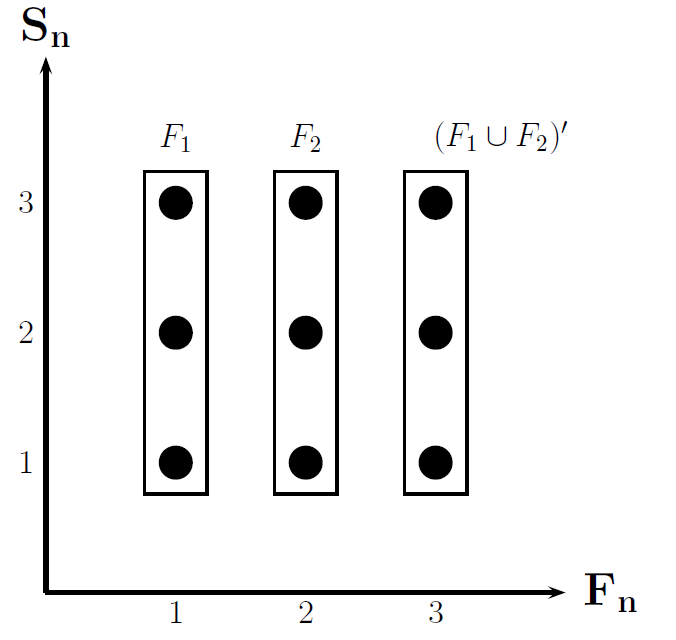
\includegraphics[width=50mm]{pictures/Prob1_2a.png}

\begin{itemize}
	\item Mutually exclusive
	\item Collectively exhaustive
	\item Event space
	\item Not sample space
\end{itemize}
\end{multicols}
\end{enumerate}
}


\frame{
\frametitle{Problem 2}
\begin{enumerate}
\item[(b)] $F_1 \cap S_1$; $F_1 \cap S_2$; $F_2$; $F_3$; 
\begin{multicols}{2}
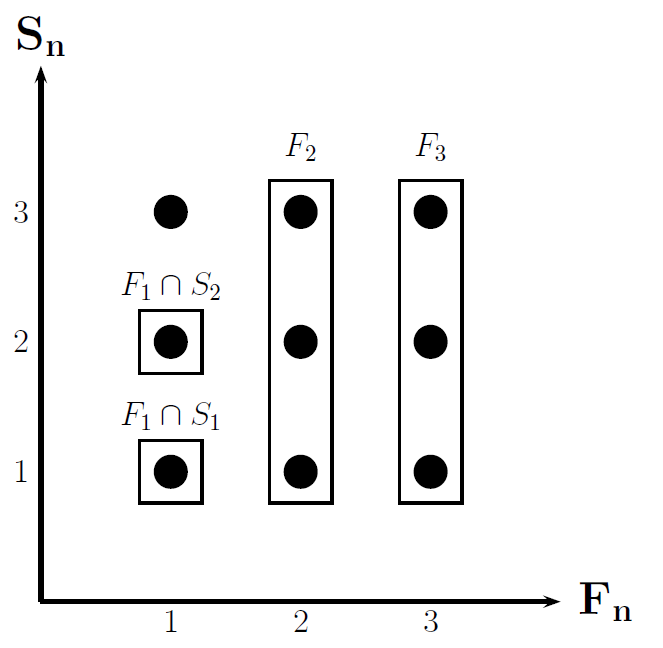
\includegraphics[width=50mm]{pictures/Prob1_2b.png}

\begin{itemize}
	\item Mutually exclusive
	\item Not collectively exhaustive
	\item Not event space
	\item Not sample space
\end{itemize}
\end{multicols}
\end{enumerate}
}


\frame{
\frametitle{Problem 2}
\begin{enumerate}
\item[(c)] $F_1 \cap (S_2\cup S_3)$; $(F_1)'$; $(S_1 \cup S_2)'$
\begin{multicols}{2}
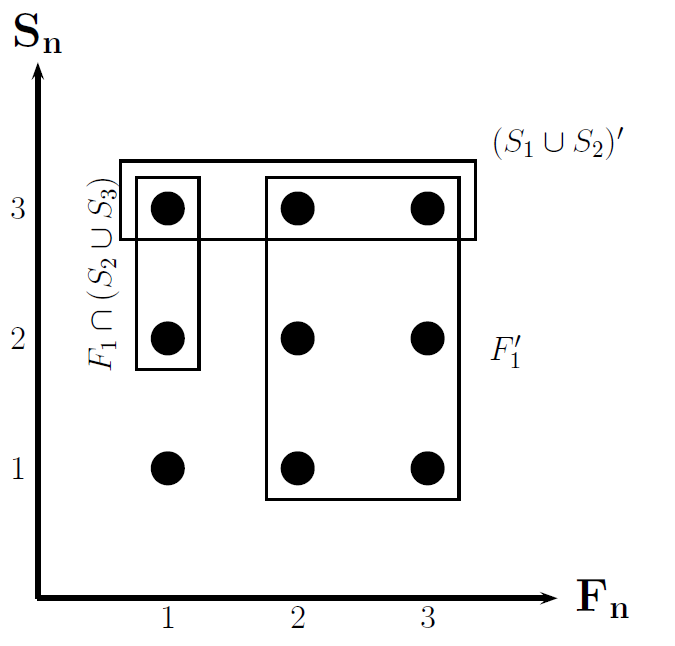
\includegraphics[width=50mm]{pictures/Prob1_2c.png}

\begin{itemize}
	\item Not mutually exclusive
	\item Not collectively exhaustive
	\item Not event space
	\item Not sample space
\end{itemize}
\end{multicols}
\end{enumerate}
}



\frame{
\frametitle{Problem 2}
\begin{enumerate}
\item[(d)] $(F_1 \cup F_2) \cap (S_1 \cup S_2 \cup S_3)$; $(F_1 \cup F_2) \cap S_3$; $F_3 \cap (S_1 \cup S_2 \cup S_3)$; $S_3 \cap F_3$
\begin{multicols}{2}
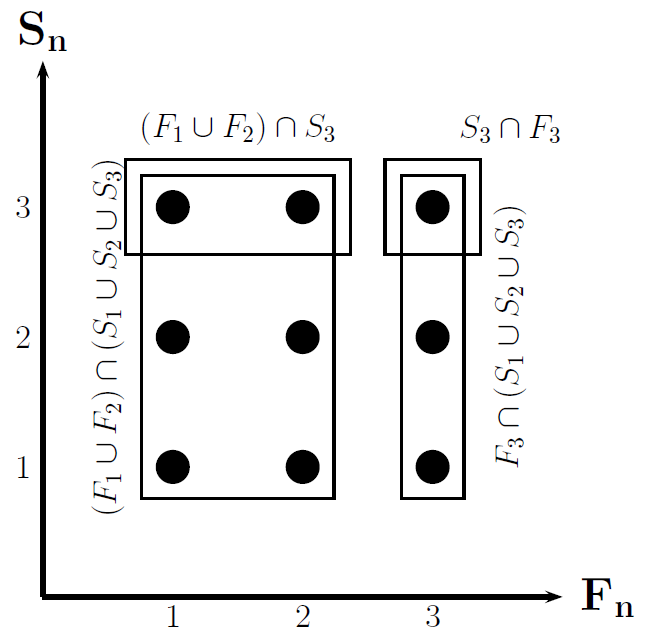
\includegraphics[width=50mm]{pictures/Prob1_2d.png}

\begin{itemize}
	\item Not mutually exclusive
	\item Collectively exhaustive
	\item Not event space
	\item Not sample space
\end{itemize}
\end{multicols}
\end{enumerate}
}


\frame{
\frametitle{Problem 3}
Answer and fully explain your answers to the following three questions (15 marks, 5 each):
\begin{itemize}
\item[(a)] If events $E$ and $F$ are mutually exclusive but not collectively exhaustive, are $E'$ and $F'$ collectively exhaustive? \\ \emph{Yes. Say, $S=\{E,F,G\}$ then $E'=F+G$, $F'=E+G$, it follows $E'+F' = E+F+G$.}
\item[(b)] If events $E$ and $F$ are mutually exclusive and collectively exhaustive, are $E'$ and $F'$ mutually exclusive? \\ \emph{Yes. Say, $S=\{E,F\}$ then $E'=F$ and $F'=E$.}
\item[(c)] If events $E$ and $F$ are not mutually exclusive but are collectively exhaustive, are $E'$ and $F'$ collectively exhaustive? \\ \emph{No. Say, $S=\{E,F\}$ where $E=\{1,2,3\}$ and $F=\{3,4,5\}$ then $E'=\{4,5\}$ and $F'=\{1,2\}$.}
\end{itemize}
}

\frame{
\frametitle{Problem 4}

Only three parties, Conservatives, Labour, and Liberal Democrats, face off in a parliamentary election (10 marks, 5 each).
\begin{enumerate}
\item[(a)] Ignoring the possibility of ties, what is the sample space of such an example of an election?
\item[(b)] A minority or coalition government must be formed if it is not the case that one party gained a majority of votes. What is the probability that the government can be formed without the need for a minority or coalition government?
\end{enumerate}
}

\frame{
\frametitle{Problem 4}
Two possibilities for winning. Either by majority or by plurality. \\
\begin{enumerate}
\item[(a)] Sample space: 
	\begin{enumerate}
	\item[1.] \{$C_m$; $L_m$; $LD_m$; $C_p$; $L_p$; $LD_p$\} 6 outcomes
	\item[2.] \{$C_m$,$L_2$; $C_m$,$LD_2$; $L_m$,$C_2$; $L_m$,$LD_2$; $LD_m$,$C_2$; $LD_m$,$L_2$; \\
	$C_p$,$L_2$; $C_p$,$LD_2$; $L_p$,$C_2$; $L_p$,$LD_2$; $LD_p$,$C_2$; $LD_m$,$L_2$\} 12 outcomes
	\end{enumerate}
\item[(b)] Probability of having a government with a majority (no plurality):
	\begin{enumerate}
	\item[1.] \{$C_m$; $L_m$; $LD_m$\} 3 ways over 6 outcomes: \emph{Prob} = 0.5
	\item[2.] \{$C_m$,$L_2$; $C_m$,$LD_2$; $L_m$,$C_2$; $L_m$,$LD_2$; $LD_m$,$C_2$; $LD_m$,$L_2$\} 6 ways over 12 outcomes: \emph{Prob} = 0.5
	\end{enumerate}
\end{enumerate}
}

\frame{
\frametitle{Stata and R session}
\begin{center}
Loops, functions and programs in Stata and R
\end{center}
}

\frame{
\frametitle{Math refresher (part 1)}
\begin{enumerate}
\item Notation
	\begin{enumerate}
	\item Variables and constants
	\item Sets
	\item Operators
	\end{enumerate}
\item Linear algebra
	\begin{enumerate}
	\item Scalars
	\item Vectors
	\item Matrices
	\end{enumerate}
\item Functions
	\begin{enumerate}
	\item Basic definitions
	\item Properties
	\item Important functions
	\end{enumerate}
\end{enumerate}
}

\frame{
\frametitle{Math refresher (part 2)}
\begin{enumerate}
\item[4.] Calculus
	\begin{enumerate}
	\item[4.1] Basics
	\item[4.2] Limits
	\item[4.3] Derivative
	\item[4.4] Rules of differentiation
	\item[4.5] Extrema
	\end{enumerate}
\item[5.] Integrals
	\begin{enumerate}
	\item[5.1] Definite integral
	\item[5.2] Indefinite integral
	\item[5.3] Fundamental theorem of calculus
	\item[5.4] Rules of operation
	\end{enumerate}
\end{enumerate}
}

\frame{
\frametitle{Conclusion}

\begin{center}
All clear? Questions? \\
Thanks and see you next week!
\end{center}
}


\end{document}
